\section{Motivation and Background}
\label{background}

Single GPU performance has been scaling very well amassing a significant
growth in per-GPU transistor count and DRAM BW. For example a 2010 Nvidia's
529mm\textsuperscript{2} Fermi GPUs integrated 1.95B transistors with 180 GB/s
DRAM bandwidth, while 2016 Nvidia 610 mm\textsuperscript{2} Pascal GPUs reached
a 12B transistor count with 720 GB/s memory bandwidth. Unfortunately transistor density
growth slows down and expected to come to a halt at 7nm. Moreover, as GPU die sizes
have been also increasing over the past generations, this growth is expected to
slow down due to limitations in lithography and manufacturing costs. 
Without larger or denser dies, GPU manufacturers are likely to turn to 
alternative technologies such as the tried and trued solution from CPU world,
the \textit{multi-socket GPUs}, to keep scaling effective GPU perfromance via 
growing overall transistor counts and DRAM bandwidths. 

%One moving to 3D die-stacking as a solution for continued transistor growth. 
%Unfortunately 3D die-stacking still has a significant number of engineering 
%challenges related to power delivery, energy density, and 
%cooling~\cite{verbree2010cost} when employed in maximal die-sized chips such as 
%GPUs and moving beyond a 2 high stack to 4 or 8 stacks will be even more 
%difficult. Because of these challenges, 
%GPU manufacturers are likely to 
%consider a tried and trued solution in the CPU world to gain additional 
%transistor count, \textit{multi-socket GPUs}.

\begin{figure*}[tp] 
    \centering
    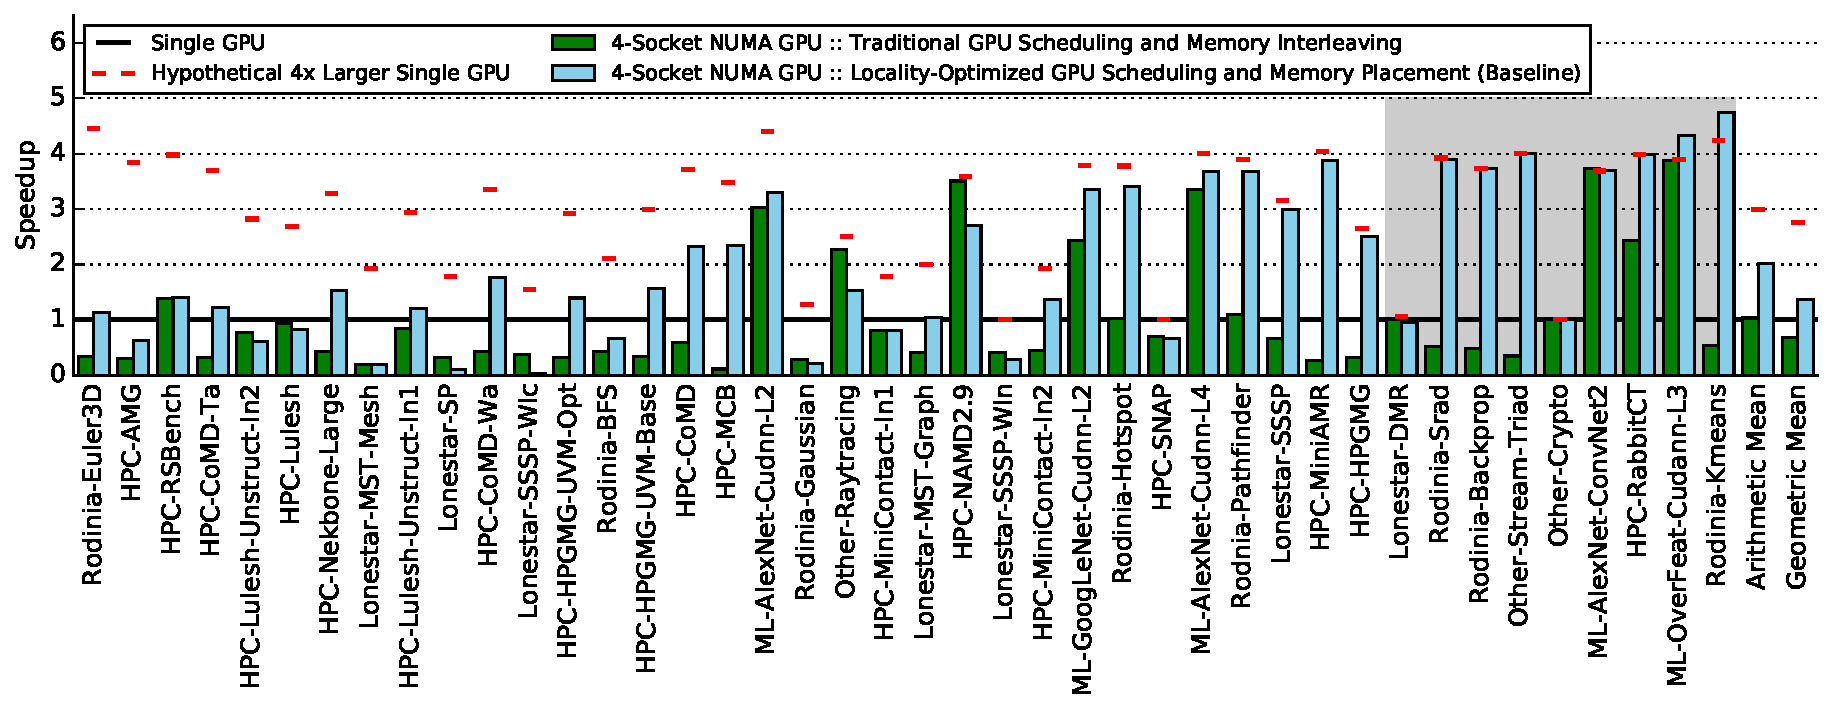
\includegraphics[width=1.0\linewidth]{figures/plot_different_baselines.pdf}
    \caption{Relative performance of a 4-socket NUMA GPU using to a single GPU 
and a hypothetical 4$\times$ larger (all resources scaled) single GPU showing 
upper bound of performance this application can achieve via GPU hardware 
scaling. For the Locality-Optimized design, applications shown in grey 
achieve already 99\% of theoretical scaling (\emph{red dash}) without 
microarchitectural modification.}
    \label{fig:motivation}
\end{figure*}

The evolution of GPU computing has moved from it being a PCIe attached peripherals 
to computing platforms designed around the GPU as the primary computing engine. 
Such systems epmloy custom PCB designs that accommodate multiple high pin count socketed 
GPUs~\cite{DGX} with inter-GPU interconnects resembling QPI or 
Hypertransport~\cite{INTELQPI,AMDHT} much more than legacy PCIe interfaces.  
Despite the improvement in hardware capabilities, to-date these multi-GPU 
solutions have been exposed as a collection of single GPU solutions with improved GPU--GPU 
interconnects. While multi-GPU systems can provide high aggregate throughput, 
the programming models for multi-GPU systems has diverged from the single GPU 
programming model and requires layering additional software runtimes like MPI 
or openshmem on top of the native GPU programming interfaces such as CUDA or openCL.
By requiring re-writing of the GPU application to enable multi-GPU performance, 
many applications are never ported to use multiple GPUs.

In this work, we examine the performance achievable by architecting a 
multi-socket NUMA-aware single GPU.  Building upon existing work in the 
NUMA-CPU and GPU community, we first describe the basic multi-socket GPU runtime 
that allows a multi-socket GPU system to be exposed to GPU developers as a 
single GPU and exploits some well known scheduling and memory locality 
optimizations for NUMA systems. We then look at the performance implications 
that this multi-socket NUMA design has on applications that have been optimized 
for a traditional single GPU.  We identify that current GPU interconnect 
utilization and cache policies are sub-optimal for a multi-socket NUMA GPU and 
show how these problems can largely be overcome with architectural innovation.  
Finally, we examine the scaling efficiency of a multi-socket NUMA-aware GPU to 
understand if NUMA-aware GPUs will see significantly improve performance  
without any code-rewriting required by the application programmer.
\\\\
\textbf{A Multi-Socket GPU Runtime}
\\\\
\noindent As demonstrated by Cabezas et al.~\cite{Cabezas2015} it is possible 
to design a framework and a runtime system that transparently decomposes GPU 
kernels in sub-kernels and executes them on multiple GPUs in parallel. On the 
Nvidia GPUs, this is doable by intercepting and remapping each single kernel 
call, GPU memory allocation, GPU memory copy and GPU wide synchronization issued 
by the CUDA driver. Special care needs to be put (i) to the GPU local memory 
fences which needs to be promoted to system level and (ii) to the 
sub-kernels CTA identifiers which needs to be properly corrected to 
reflect those in the original kernel call. 
 
In ~\cite{Cabezas2015} these two problems were solved by introducing  
code annotations and an additional source-to-source compiler which was also 
responsible for statically assigning data and computation on each GPU. In our 
work, we follow a very similar strategy but we do not use any additional 
compiler for two reasons (i) we use a simulated environment in which 
we can properly model the architectural requirements for system wide memory 
fences and sub-kernel to kernel CTA identifiers mapping (ii) we model a system 
which implements UVM page migration on demand, as recently introduced in the 
Tesla P100 GPU~\cite{P100}. UVM page migration allows to allocate 
all the memory upfront in system memory and to transparently migrate pages 
on the GPU memory on demand as soon as the first access (also called first 
touch) is performed.

Another approach for memory placement is to mimic what a single GPU does, 
which is to interleave memory at the granularity of single cache line to 
reduce memory camping effects and to maximize bandwidth. However interleaving 
at such fine granularity across multiple GPUs disrupts locality and it 
results in large amount of remote accesses even for regular and dense 
applications. A less fine grain solution is to interleave memory across GPUs 
at the granularity of pages. With respect to kernel partitioning, while on a 
single GPU fine grain dynamic assignment of CTAs to the SMs is performed to 
achieve good load balancing, extending it to a Multi-GPU system (for instance 
creating a large amount of small sub-kernels) results in huge overhead due to 
the cost of starting a single sub-kernel. For this reason, as done 
in~\cite{Cabezas2015}, we decompose a single kernel in only N sub-kernels, 
where N is the total number of GPUs in the system, and we assign to each GPU 
an equal amount of CTAs. We also select CTAs in each sub-kernel to be 
contiguous. This last choice could expose workload unbalance across 
sub-kernels, but it preserves locality present in many dense and regular 
applications where contiguous CTAs access contiguous memory. In the attempt 
to reduce unbalance an alternative solution consists in interleaving CTAs 
across the sub-kernels trying to follow the way pages interleave across 
memories. 

In Figure~\ref{fig:motivation} we show the relative performance a 4-Socket 
NUMA GPU with respect to a single GPU for two possible CTA scheduling and 
memory placement strategies above explained (see Section~\ref{methodology} 
for a detailed explanation of methodology and benchmark suites). With the 
\emph{green bars} we show relative performance of the natural extension to 
the traditional single GPU scheduling and memory interleaving to 
multi-GPU, which consists in memory page interleave and sub-kernel CTA 
interleave. With the \emph{light blue bars} instead we show the relative 
performance of the locality optimized GPU scheduling and memory placement 
consisting of contiguous block CTA scheduling and first touch page 
migration. We can clearly see that the Locality-Optimized solution almost always 
outperforms the traditional GPU scheduling and memory interleaving, in 
average performing 2x better. In general the problems of data placement and 
task placement (minimizing remote data access and ensuring good load balancing) 
can not be completely decoupled and pathological case can always be found. It 
is important to stress that we are not claiming the Locality-Optimized solution 
as a contribution of this paper (indeed very similar considerations and findings 
can be found in~\cite{Cabezas2015,Arunkumar2017}), instead we are setting up a 
baseline architecture in which we can apply and present our proposed 
optimizations in the next Sections.

Also in Figure~\ref{fig:motivation} we show with a \emph{red dash} the performance 
achievable by an hypothetical (unrealizable) 4x larger GPUs. This \emph{red dash} 
represent a good approximation of the maximum theoretical performance we 
could expect from a perfect NUMA system. We sorted the applications by the 
gap between relative performance of the Locality-Optimized and 
Hypothetical 4x larger GPUs. We can see that on the right side of the graph 
some applications (that have very good locality) already 
achieve or surpasses the maximum theoretical performance. In particular for the 
two far-most benchmarks on the right, the locality optimized solution outperforms 
the hypothetical 4x larger GPU due a better reuse of L2 data originated by 
the contiguous block scheduling of CTAs. For the applications on the left 
side of the Figure there is quite large gap between locality optimized and 
hypothetical. These are the applications in which either, locality does not 
exists or the Locality-Optimized solution can't capture it, 
resulting in large amount of remote transfers. In the rest of this paper we 
present techniques aimed to reduce this gap. To simplify the discussion we 
will exclude the benchmarks that already achieve 99\% of the theoretical 
performance when explaining these techniques. We will re-include them in the 
final plots to demonstrate that there was not performance regression due to 
our proposed optimizations.
